\documentclass[11pt]{ECEtemp}

%%%%This is where you change your Name.Assignment.Class.etc...
\newcommand{\assignment}{Title (Chapter One Homework)}
\newcommand{\subdate}{April 29, 2019}
\newcommand{\class}{EE-2263  -  Embedded Systems}
\newcommand{\Name}{Your Name, left justified, 11 or 12 pt. type}
\newcommand{\prof}{Dr. Nathan Hutchins}

\lstset{language=c}

\begin{document}
%%%Set up of the Name Section
\noindent
\Name \\ \class \\ \prof \\ \subdate 
%%%This places your title
\eceTitle{\assignment}
%%%Here is your report start! Good Luck!

\eceSection{Objective, Heading 1, Black lettering}
Describe the objective of the assignment or report. This includes the purpose of the report and a brief description of the results to be reported. For example: This template provides guidance on formatting and organizing a laboratory or design report to make the report more readable and more informative, and to abide more closely with the standard reporting formats of industry.

\eceSection{Introduction, (for design reports)}
Describe in a paragraph or two what you are doing and why you are doing it, to give the reader enough background to understand what they are about to read.  For example:

An important aspect of an engineer’s job consists of effectively communicating the results of experiments, simulations, and/or theoretical investigations to their peers, management, and potential or current business partners and collaborators. Engineer’s skilled in effective communication are more valued by their company or organization in general. This report describes a general method for organizing and presenting information that will enhance the user’s ability to effectively communicate their work.

\eceSection{Equipment or Tools Used}
\begin{itemize}
\itemsep0em %Reduce the space between items of the list!
\item   ECLIPSE with MinGW
\item   CLion with Clang
\item   Terminal with GCC
\end{itemize}

\eceSection{Methodology}
\noindent 1. Design requirements (design report) or Specific Objectives (lab report)
\begin{enumerate}[(a)]
    \itemsep0em %Reduce the space between items of the list!
    \item Create a design report that is well-organized, comprehensive, and easy to read
    \item Read Chapter 1 and complete the required assigned problems.
\end{enumerate}

\noindent 2. Description of Design Process (design report) or Sequence of Measurement/Analysis (lab report)

In this section, describe in a logical order how you proceeded in designing, analyzing, and/or measuring the project element or element(s). This section can consist of word descriptions, tables, equations and figures.

\eceSection{Results}

Put your results here, be sure to include flowcharts, Code snips, descriptions, console/file output. Give me everything you have, I don't take away points for reports that are to long, but I take a lot for reports that are too small.

\begin{figure}[!htb]
    \centering
    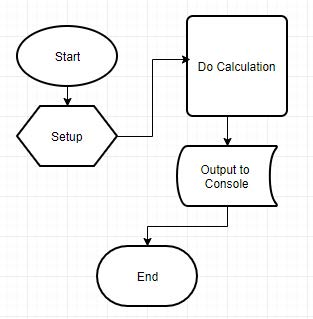
\includegraphics[scale=1]{img/fig_flowchart.jpg}
    \caption{Flow Chart}
    \label{fig_figure_1}
\end{figure}

Using flow charts will help you design your program as well as help me follow what you were trying to do. Flow charts are easy in the beginning but get harder as we go along. Use draw.io to create your flow charts.

\begin{figure}[!htb]
    \centering
\begin{lstlisting}
struct student {
    char studentName[20];
    char studentDegree[20];
    int studentAge;
    float studentGpa;
};
\end{lstlisting}
    \caption{Code Section}
    \label{code_snip1}
\end{figure}

Having code snips in your discussion to show specific issues, or creative solutions goes a long way for making a report feel good, and not be boring.

\begin{figure}[!htb]
    \centering
    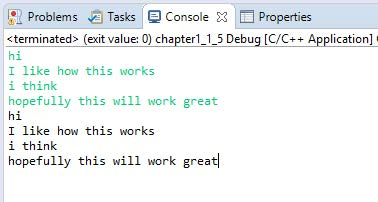
\includegraphics[scale=1]{img/fig_console_output.jpg}
    \caption{Console Output}
    \label{fig_figure_2}
\end{figure}

Outputs are obviously very important, I mean, did your program even work.

\eceSection{Conclusions}
Conclude your report with your conclusions and be sure to check that you are using the proper file naming scheme, LastName\_Assigment\_V0.pdf

\eceSection{Appendix}
Add any extras needed in the Appendix

\centering
\lstinputlisting{code_snips.c}


\end{document} 

